\section{Solidification, Untangling, and CT Attachment}
\label{sec:finishing}

\plain{In brief: parameterization makes defects measurable, but measurable is not the same as fixable. This section covers four operations: filling holes inside one accepted sheet; separating a surface that passes through itself; nudging geometry onto the papyrus the CT actually shows; and choosing which layer supplies each output pixel. Each accepts a change only when the geometry it produces measures better than the geometry it replaces.}

The temptation at this stage is a familiar one. Once the sheet is flat, every defect is visible and every defect looks fixable: a hole can be interpolated, a dark island can be moved to the nearest bright voxel, a raster void can be filled. Each of those operations improves the picture. Three of the four can also destroy the result, because each can silently connect material across a wrap boundary. The design here is therefore built around what each operation is forbidden to touch.

\subsection{Component-Bounded Solid Fill}
\label{sec:solidfill}

A fitted material track is single-valued over most, but not all, of its parametric bounding box. The solid-ribbon builder allocates a regular quad lattice over the union of each component's occupied row and column spans. Directly fitted vertices form Dirichlet data. Missing positions inside that component solve the four-neighbour harmonic problem
\begin{equation*}
  x_i = \frac{1}{|N(i)|}\sum_{j\in N(i)} x_j,
  \qquad i\in\mathcal H_c,
\end{equation*}
independently for each world-coordinate component, with a sparse direct solve for small holes and preconditioned iteration for larger ones. A cylindrical alternative continues radius and lifted phase under the same boundary conditions, using local pitch to preserve turn order.

The single most important property of this operator is negative: the fill domain $\mathcal H_c$ never crosses a component label. Separate tracks, separate wraps, and quarantined order claims remain separate even where filling the rectangle between them would produce a visibly more complete image. A neighbour carrying another component label is simply not in the stencil, and there is no inter-component fill state anywhere in the implementation.

On an early full-grid implementation this operation added 18.8\% support on $4\times5\times5$ and 15.8\% on $10\times10\times10$, with approximately zero dark pixels and 0.04\% multiple coverage in the immediate structured bake. Those aggregate numbers turned out to be insufficient, and the reason is worth recording: generated continuation can look geometrically regular while crossing a wrap that the \emph{source prediction} had already fused. The fill was locally correct and globally wrong, and no measurement of the fill itself could tell. We therefore retain direct and filled labels through every subsequent measurement, and never report full-rectangle quality without a support-masked companion.

\subsection{Exact Collision Untangling}
\label{sec:untangle}

\plain{In brief: a coiled ribbon fitted from noisy observations will, in places, pass through itself. That is physically impossible, and no amount of CT-guided correction can repair it, because the two interpenetrating layers are competing for the same voxels.}

The untangler first applies a sparse turn-order escape, then builds an \emph{exact} triangle-contact set --- exact pairwise tests, not raster occupancy, because occupancy at any practical resolution cannot resolve two sheets 7 voxels apart. Each contact identifies two continuous phase branches and their radial order. A scalar radial displacement field is then solved over an active collar with screened parametric smoothness, unilateral inter-turn clearance, and the pre-escape ribbon as a rest shape. Every trial is tested for exact pair intersections, folds, and orientation reversals.

One scheduling detail is load-bearing. Temporary growth in the contact count is accepted, but only while the number of \emph{phase-order violations} falls. Without that allowance an intersection curve is pinned at whichever triangle pair it first touched and can never travel across the tessellation to a configuration where it can be removed; the measured sequence on the first 15\% diagnostic is $428\rightarrow2{,}138\rightarrow7{,}630\rightarrow104\rightarrow0$, and a monotone acceptance rule stalls permanently at 428. Once long contacts are cleared, a settle phase pulls the ribbon toward its measured rest coil while enforcing every accumulated contact.

On that diagnostic, sparse repair alone stalls at 428 long contacts and four elastic-shell steps reach zero with no folds. After two guarded CT passes and metric relaxation the crop contains two benign local overlap classifications, zero stabs, and zero folds. A confidence-preserving coarse variant reduces the working mesh to 8.39\% of its vertices, lowers the solve from 39 minutes to 2 minutes 14 seconds, clears 3,496 long contacts, and ends at zero overlap, stab, and fold with Sander $p95/p99$ of 1.359/1.461.

The full $4\times5\times5$ solve takes 7 minutes 29 seconds, against 16.5 non-converged hours for the preceding method. The shell reaches its best exactly-tested state at 4,688 contacts rather than the earlier 147,728, and guarded snap reduces this to 4,073. The output has strict RAW coverage 294/294, 100\% raster coverage, and no skipped or multiply covered pixels. Its 11.53\% dark rate is 0.91 percentage points worse than the less topologically sound predecessor --- a real cost of untangling, since a sheet forced to be intersection-free gives up brightness that a self-overlapping sheet had obtained by sampling the same material twice. The shell does not reach zero on the full sheet: its 313,000-contact set becomes mutually restrictive, and contact pruning together with the newer pre-weld input are the next controlled variables.

The $10\times10\times10$ diagnostic establishes a different and more important boundary. Its fitted, measured region is strong --- dark 4.58\%, Sander $p95/p99$ 1.13/1.23, only 0.04\% at $\ge 4\times$ --- but 41\% of the full rectangle is generated continuation crossing wraps that were fused in the source prediction, and that continuation is dark 25.7\% with 30.6\% at $\ge4\times$. No untangler can recover an identity that was already destroyed upstream; those pixels remain outside the shipped mask, and the failure is attributed to the prediction rather than to the geometry.

\subsection{Transactional CT Attachment}
\label{sec:attach}

\plain{In brief: the fitted surface is a good guess at where the papyrus is, but the CT knows better. Snap moves geometry onto the measured papyrus band --- and then has to prove, against six independent measurements, that the move was an improvement.}

The first geometry is a warm start, not a set of immovable measurements. Vertices backed by direct fit evidence stay fixed; interpolated vertices, and fitted vertices touching dark emitted triangles, may move. For each active region the snapper searches within a winding-aware corridor for a coherent papyrus-band target, fits a robust vector field from the accepted targets, applies a smooth displacement, remeshes correspondences where needed, and rebakes against the authoritative RAW volume.

Two aspects of target selection deserve comment. The corridor is winding-aware, so a candidate can never be found on the far side of an intervening wrap, however bright that wrap is. And the target is a \emph{band}, an oriented dark-to-bright transition scored for local coherence, rather than an intensity maximum: papyrus placement is not an intensity-maximum problem, and a vertex that chases the brightest nearby voxel will happily walk off its own sheet.

\paragraph{The accept/reject rule.} A pass is committed only when it satisfies \emph{all} of the following relative to its input state: no new orientation violation; no growth in the contact set; no multiple coverage and no raster hole; no fixed-window darkness regression outside an explicit Pareto allowance; and no material Sander-distortion regression. A candidate can therefore improve CT intensity --- the thing one is most tempted to optimize --- and still be rejected.

The loop is iterative and component-selective. The outer loop rebakes the accepted state, detects broad residual black regions, proposes releasing only their suspect evidence, and evaluates each component independently. A rejected component remains bit-identical to its previous state; accepted and rejected components are then rebuilt into one mixed monolith. Correspondence remeshing is likewise objective-selected rather than mandatory. The process stops when no component proposal passes, which makes the terminal state a \emph{measured fixed point} rather than a chosen round count --- a distinction that matters, because a hand-selected iteration count is indistinguishable from stopping when the picture looked best.

\paragraph{Result.} The $4\times5\times5$ V83 fixed point contains 4,100,366 unique vertices and 8,168,120 faces. Its independently baked fixed-window texture has 258,276 dark pixels (3.162\%), Sander $p95/p99$ 1.190/1.380, 11,142 samples at $\ge2\times$, 428 at $\ge4\times$, and zero UV skips, 3-D skips, multiple coverage, enclosed holes, or coverage faults. Relative to V67 it removes 768 dark pixels, 323 $\ge2\times$ samples, and 78 $\ge4\times$ samples. One further proposal round leaves every previously rejected component byte-identical except one, and that component worsens darkness and both distortion tails and is rejected --- which is what convergence looks like when it is measured rather than declared.

\begin{figure*}[t]
  \centering
  \begin{subfigure}[b]{0.98\linewidth}
    \centering
    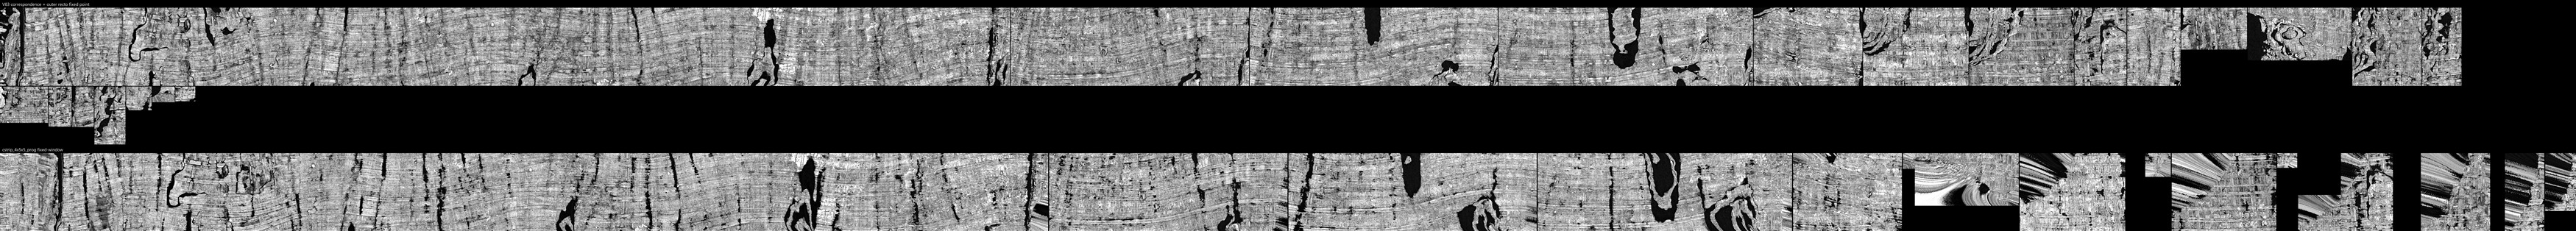
\includegraphics[width=\linewidth]{figures/quadribbon_v83_vs_progressive_raw.jpg}
    \caption{Fixed-window RAW comparison: V83 (top) and the progressive baseline (bottom).}
  \end{subfigure}
  \medskip
  \begin{subfigure}[b]{0.98\linewidth}
    \centering
    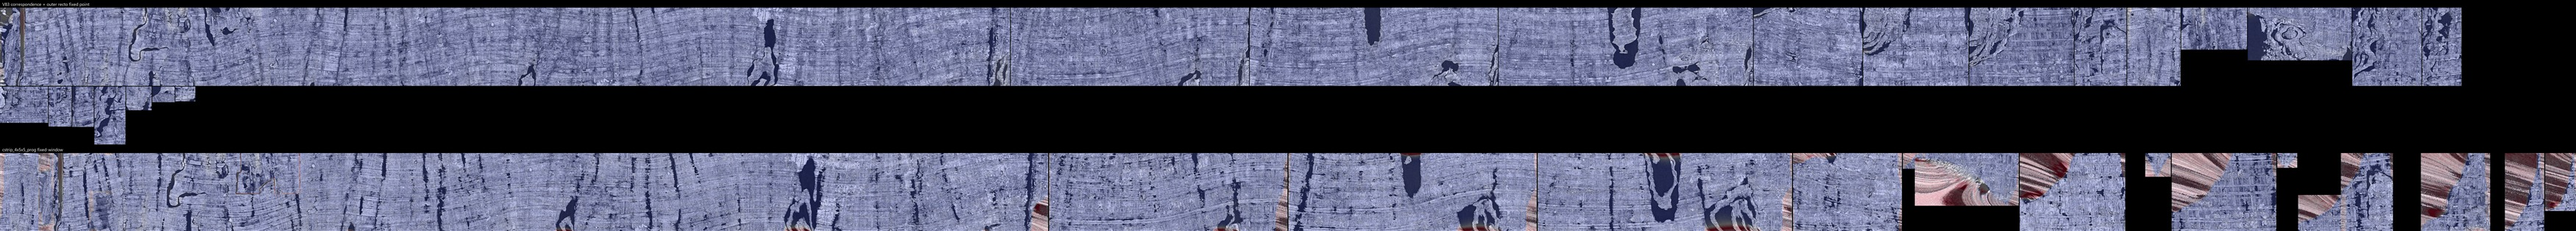
\includegraphics[width=\linewidth]{figures/quadribbon_v83_vs_progressive_sander.jpg}
    \caption{The corresponding Sander distortion view; red tails concentrate in the baseline's folded continuation.}
  \end{subfigure}
  \caption{Transactional solid-ribbon result. Against the same RAW source, the mature V46/V83 lineage lowers dark area, eliminates multiple coverage, and reduces the $\ge4\times$ distortion population by roughly $320\times$ relative to the progressive baseline; V83 then supplies the measured convergence point of the residual loop.}
  \Description{Two very wide paired strip images. The upper pair shows grayscale papyrus textures; the lower pair overlays distortion colors, with more red regions in the baseline row.}
  \label{fig:recto-fixed-point}
\end{figure*}

\subsection{Raster Correctness, Layering, and Output Masking}
\label{sec:raster}

\paragraph{Sampling.} The rasterizer samples pixel centres. The first exact-metric ribbons exposed a half-texel bounding-box error: enumerating a triangle from $\lceil u_{\min}-0.001\rceil$ is correct for historical integer-lattice UVs but drops the first row or column of faces at generic sub-voxel phase. The correct bound is $\lceil u_{\min}-0.501\rceil$. On the $4\times5\times5$ metric sheet the fix reduces bounded void-fill from 1,268,329 pixels to 3,707 while remaining bit-identical on integer-lattice tests. The episode is a useful illustration of why void-filling is dangerous as a default: the bug had produced a smooth, plausible, entirely false green smear over a million pixels of real geometry, and only the discrepancy between two representations exposed it.

\paragraph{Layers.} Where the papyrus has delaminated, two plies legitimately occupy nearly the same $(u,v)$, and both are real. Hard layer conflicts --- overlap exceeding 5\% of the smaller chart --- are separated into distinct sheet bakes; soft boundary kisses remain in the primary sheet but are recorded edge by edge. The final first-cover composite prefers direct coverage from any layer over an earlier layer's generated fill, and writes a per-pixel label. On the fixed-topology $4\times5\times5$ result, secondary layers recover 389,628 pixels the primary alone misses and occlude 1.25 million pixels of genuine duplicated ply coverage; every face is retained in a layer manifest, so nothing is discarded, only ranked.

\paragraph{The output mask.} Fitted pixels are kept unconditionally. A \emph{filled} pixel is kept only when the final bake classifies it as papyrus and its Sander distortion is below 2 --- its final measured state decides, not the fact that a PDE produced coordinates for it. Islands smaller than 64 pixels are removed as pepper, and the innermost region below radius 64 is excluded regardless of appearance, because pitch is not measurable there and the winding coordinate of Equation~\eqref{eq:winding} is consequently undefined.

This policy yields 83.2\% coverage, 3.02\% dark, and no $\ge4\times$ pixels on $4\times5\times5$. On $10\times10\times10$ it yields 70.1\% coverage --- at parity with the previous 70.6\% supported sheet --- while improving dark from 4.58\% to 3.59\%, Sander $p95$ from 2.73 to 1.45, and the $\ge4\times$ tail from 2.53\% to 0.03\%. The full rectangle is retained beside the mask as a diagnostic. It is never the sole deliverable.
